\graphicspath{ {LiteratureStudyImages/} }

\chapter{Literature Study}
\label{cha:literatureStudy}

\section{Introduction}
In this chapter 


\section{Background Knowledge}
We assume a basic knowledge of general computer science concepts as algorithms, time complexity, linear algebra, basic graph theory, optimization, and heuristics.


	\subsection{Machine Learning}
Machine learning is a data driven approach with as goal to build a model which can be	used to make predictions or decisions. This task is done by algorithms which are able to learn models based on examples given by the designer. In machine learning there are $3$ types of problems, namely supervised learning, unsupervised learning, and reinforcement learning. \\
Supervised learning is concerned with the learning task where there are examples given with their corresponding label. Unsupervised learning is similar to supervised learning only no labels are given. We won't go into reinforcement learning. \\
We can also classify to problems according to the desired output of our model. Those main tasks consist of classification, regression, clustering, and dimension reduction.
	
	
	\subsection{Time Series Analysis}
A time series consists of data points over a certain time period. We refer to this as a sequence of states. Where a state represents a data point and can differ from a single value to more complex representations like pictures. \\
The domain of time series analysis handles around extracting information or relations from a time series. It can have different goals like forecasting, classification, or exploratory.
	
	
	\subsection{Neural Networks}
	
A neural network is a machine learning approach based on biological neural networks. The basic component of a neural network is a perceptron. A perceptron take multiple binary inputs and has a single binary output (see figure \ref{fig:perceptron}). Each input has a corresponding real numbered weight. The output is decided on the following equation:

\begin{equation} 
output =
  \begin{cases}
    0       	& \quad \text{if } \sum_j w_jx_j \leq \text{ threshold}\\
    1  		& \quad \text{if } \text{if } \sum_j w_jx_j > \text{ threshold}\\
  \end{cases}
\end{equation}
	
\begin{figure}[H]
	\centering
	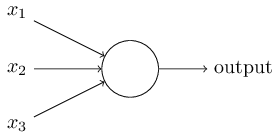
\includegraphics[width=8cm]{perceptron.png}
	\caption{A simple presentation of a perceptron.}
	\label{fig:perceptron}
\end{figure}

We can build a network by connecting multiple perceptrons (see figure \ref{fig:multiplePerceptrons}. By building these networks, more complex decisions can be made.

\begin{figure}[H]
	\centering
	\includegraphics[width=8cm]{mulitplePerceptrons.png}
	\caption{A more complex network made by connecting multiple perceptrons.}
	\label{fig:multiplePerceptrons}
\end{figure}

http://neuralnetworksanddeeplearning.com/chap1.html

\section{A Second Topic}
\lipsum[64]

\subsection{Another item}
\lipsum[56-57]

\section{Conclusion}
The final section of the chapter gives an overview of the important results
of this chapter. This implies that the introductory chapter and the
concluding chapter don't need a conclusion.

\lipsum[66]

%%% Local Variables: 
%%% mode: latex
%%% TeX-master: "thesis"
%%% End: 
